% !TEX root = ../VPJ.tex

\chapter{Visualisierung}
\label{sec:Visualisierung}

Die Auftragsplanungssoftware besitzt neben der Logik eine Visualisierung. Diese wurde mit den von Qt bereitgestellten Widgets grafisch programmiert und in der Funktion mainwindow verknüpft und organisiert. 

\section{Design}

Die Leitlinie des Grafikdesigns der HAW war:

\begin{quote}
"`Fokussiert. Direkt. Verständlich.
Und vor allem sympathisch."'	

"`Idee der neuen visuellen Sprache ist die Reduktion auf das
Wesentliche. Ziel soll es sein, einfach und klar die wichtigste
Aussage zu kommunizieren."'
\cite[4]{corporate}
\end{quote}

Beim Design der Software wurde versucht diese Aspekte wieder aufzugreifen. Die Visualisierung sollte ebenso direkt und verständlich sein. Vor allem die Reduktion auf das Wesentliche lag besonders im Fokus. 

Um die Visualisierung im Stil der HAW zu gestalten wurde das Corporate Design bei Farb und Schriftwahl verwendet. Somit sind alle Schriftarten in der Visualisierung Open Sans. Als Farben wurden die vorgegebenen Farbstile "`HAW Hauptblau"' als Umrahmung und Abtrennung aller Bereiche gewählt. Das "`HAW Hellblau"' ist innerhalb der verschiedenen Bereiche als Trennung der Bedienelemente zu sehen. Da dieses blasser ist können alle Bedienelemente gut erkannt und verwendet werden. 

\begin{figure}[htb]
    \centering
    
\includegraphics[width=0.3\textwidth]{Abbildungen/VPJ.png}
    \caption{VPJ-Logo}		
    \label{fig:VPJLogo}
\end{figure}

Das entworfene VPJ-Logo (Abb. \ref{fig:VPJLogo}) welches in Taskmanager, Taskleiste, an oberer Bildschirmseite und zentral in der Mitte der Visualisierung zu finden ist, unterliegt ebenfalls den Richtlinien, die im Corporate Design (vgl. \cite{corporate}) festgehalten sind. 

\section{Struktur}

Die Visualisierung lässt sich in insgesamt 6 Bereiche unterteilen. Die Bereiche sind in Abbildung \ref{fig:GesamtprogrammBereiche} dargestellt. Bereich I oben links zeigt die Fertigungsstraße mitsamt Robotern, Parkplätzen und Stationen. Dieser Bereich wird folgend Live-View genannt. 

\begin{figure}[htb]
    \centering
    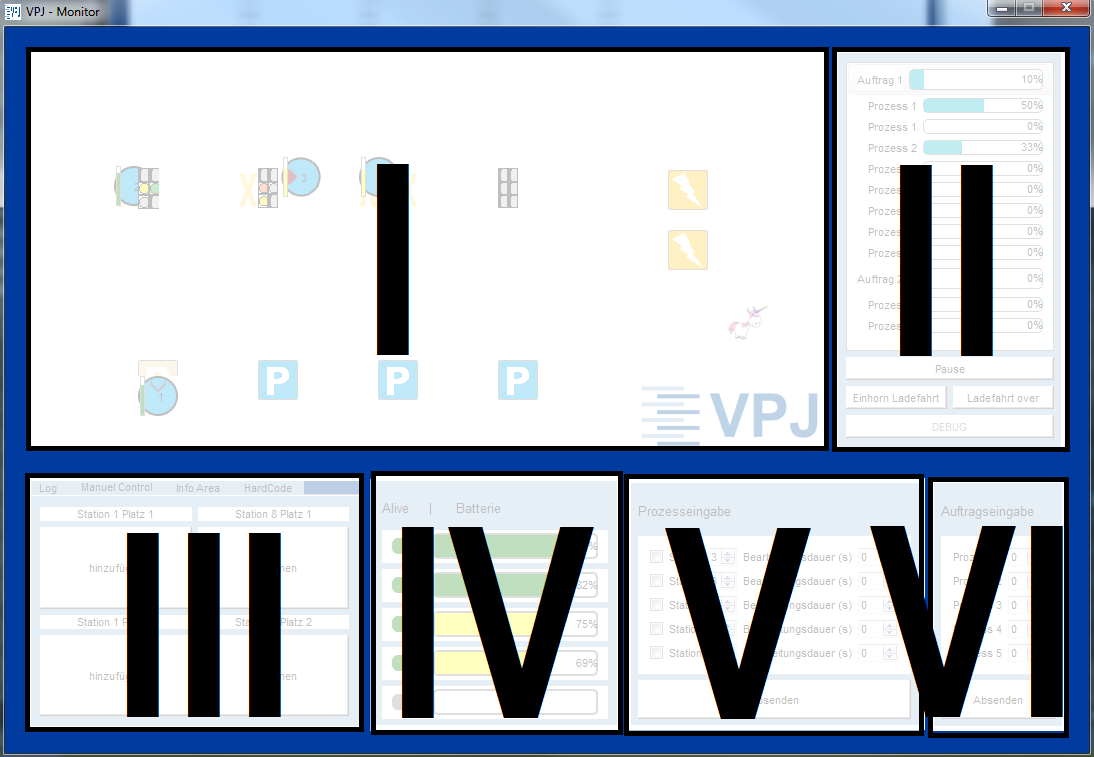
\includegraphics[width=0.8\textwidth]{Abbildungen/GesamtprogrammBereiche.png}
    \caption{Übersicht über die Bereiche innerhalb der Visualisierung}		
    \label{fig:GesamtprogrammBereiche}
\end{figure}

In Bereich II, der Auftragsübersicht, können die Fortschritte der laufenden Aufträge und Prozesse überwacht werden.

Innerhalb des Bereich III können über Tabs vier weitere Fenster aufgerufen werden. Dabei dienen zwei der Anzeige spezifizierter Informationen, wohingegen die anderen beiden Tabs der Kontrolle dienen. Die Kombination aller vier Tabs wird folgend Tab-View genannt.

Bereich IV zeigt den Status der Robotinos an. 

Die beiden Bereiche V und VI werden ausschließlich für die Erzeugung neuer Aufträge oder Prozesse verwendet. 

In Abbildung \ref{fig:Gesamtprogramm} ist eine Übersicht der Visualisierung im laufenden Betrieb dargestellt. 

\begin{figure}[htb]
    \centering
    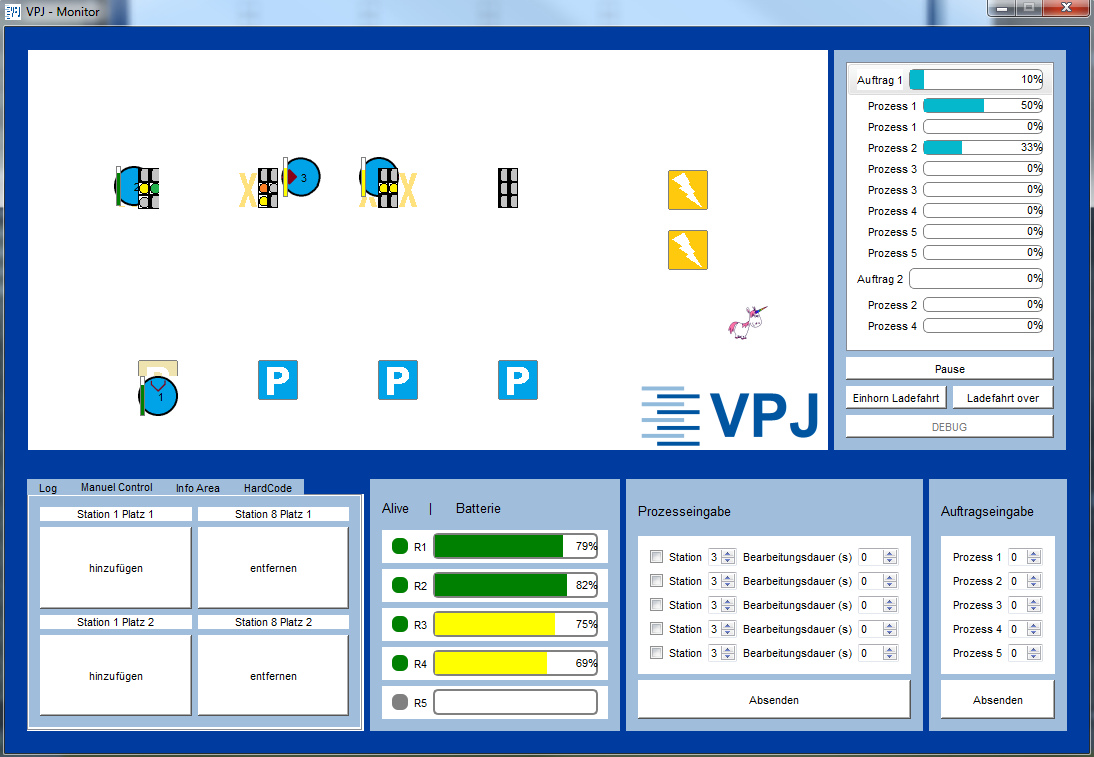
\includegraphics[width=1\textwidth]{Abbildungen/Gesamtprogramm.png}
    \caption{Übersicht Visualisierung}		
    \label{fig:Gesamtprogramm}
\end{figure}

In den folgenden Kapiteln werden die einzelnen Bereiche der Abbildung näher beleuchtet und ihre Implementierung in der MainWindow Funktion erläutert. 

\section{Live-View}

Der größte der Bereiche beinhaltet eine Live-View der Fertigungsstraße, dargestellt in Abbildung \ref{fig:LiveView}. Dabei sind alle Stationen, die Robotinos, Parkplätze und die Ladestationen dargestellt. In der unteren rechten Ecke ist das VPJ-Logo eingebettet. Das Fenster hat feste Maße von 800 x 400 Pixeln, wodurch die realen Raumabmessungen einfach dargestellt werden können. 1 Pixel entspricht im realen Raum 1 cm. 

\begin{figure}[htb]
    \centering
    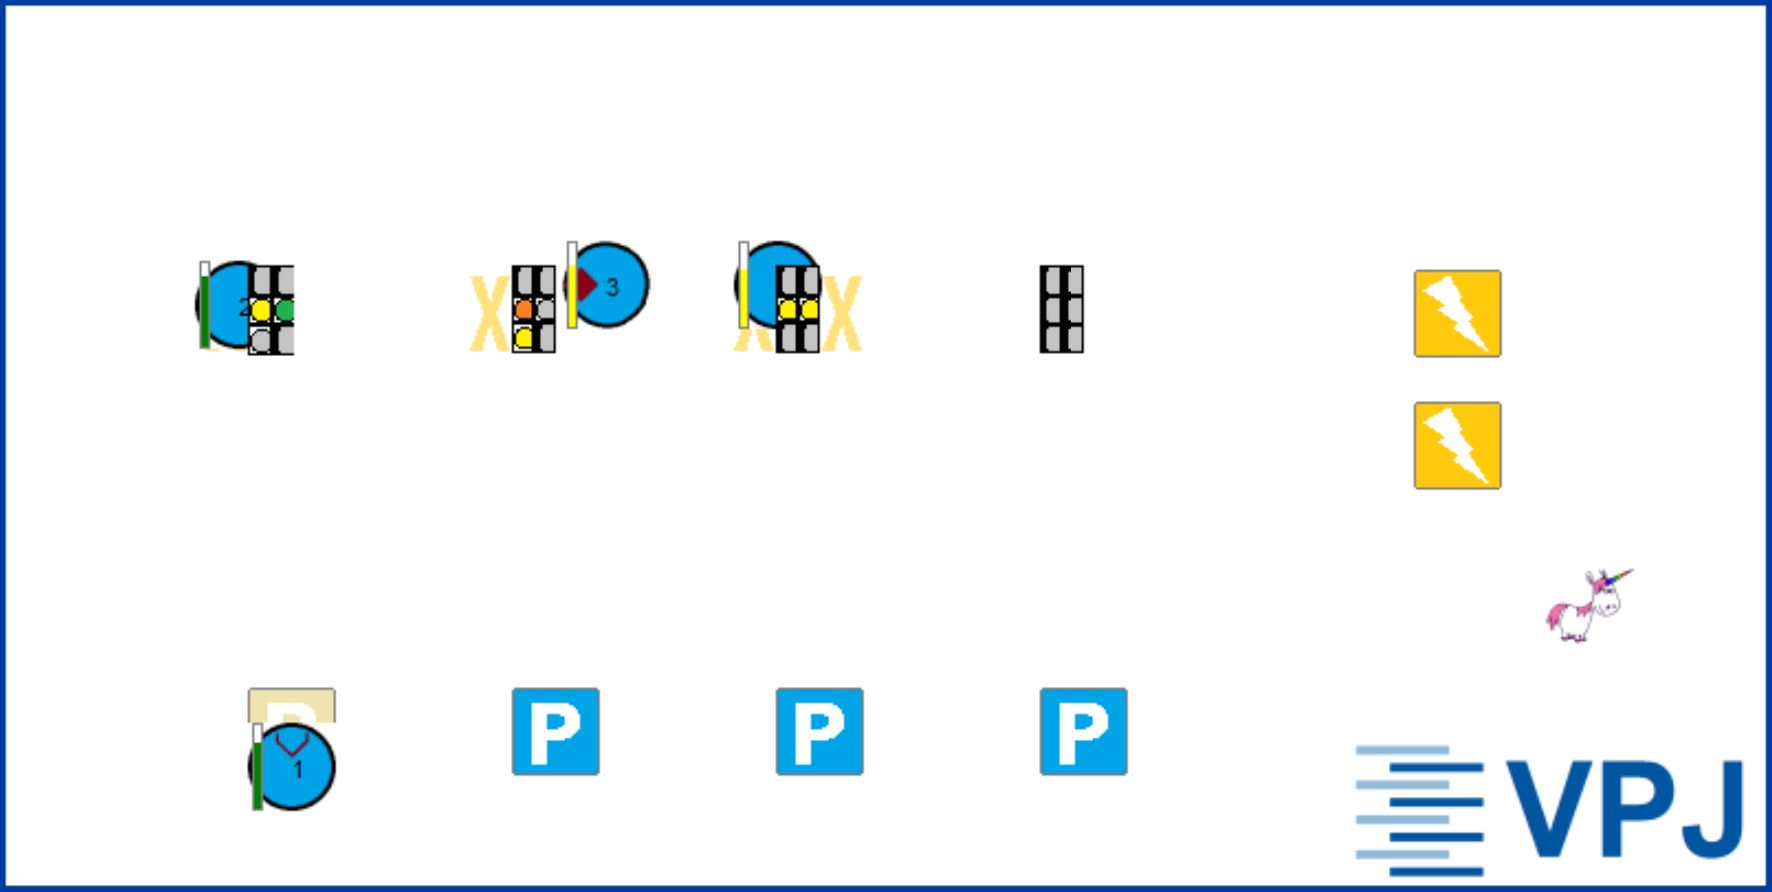
\includegraphics[width=0.9\textwidth]{Abbildungen/LiveView.png}
    \caption{Visualisierung Live-View}		
    \label{fig:LiveView}
\end{figure}

\subsection{Robotino}

Der Robotino wird immer an der Position dargestellt, die in der zugehörigen Robotinoklasse hinterlegt ist. Über die Funktion UpdateRobotinoPosition() kann eine Aktualisierung angefordert werden. Sobald der UDP-Handler neue Positionsdaten für einen Robotino empfängt und die neue Position mindestens 2 Pixel von der Alten entfernt liegt, wird diese aktualisiert. 

Die Funktion UpdateRobotinoPosition() prüft zunächst ob der Robotino ein Hindernis erkannt hat. Bei vorliegen eines Hindernis wird für den Robotino ein Bild geladen, welches im Rand den Hindernistyp kodiert. In Abbildung \ref{fig:RobotinoHindernis} sind alle auftretenden Hindernistypen dargestellt. Bei einem unbekannten Hindernis wird der Robotinorand Rot dargestellt, wie rechts abgebildet. Ein noch nicht klassifiziertes Hindernis wird, wie links abgebildet, mit gelbem Rand dargestellt. In der Mitte der Abbildung ist der Robotino mit orangenem Rand abgebildet, der bei einem anderen Robotino als Hindernis angezeigt wird.
Wenn kein Hindernis erkannt wird bleibt der Rand schwarz. 

\begin{figure}[htb]
    \centering
    
\includegraphics[width=0.12\textwidth]{Abbildungen/RobotinoGoffenRandGelb.png}
    
\includegraphics[width=0.12\textwidth]{Abbildungen/RobotinoGoffenRandOrange.png}
    
\includegraphics[width=0.12\textwidth]{Abbildungen/RobotinoGoffenRandRot.png}
    \caption{Robotino Darstellung bei verschiedenen Hinderniserkennungen}		
    \label{fig:RobotinoHindernis}
\end{figure}

Die Darstellung des Robotinos hängt neben den Hindernistypen auch von verschiedenen Stati ab. So wird ein defekter Robotino mit einer Flamme gekennzeichnet (Abb. \ref{fig:Robotino} mittig rechts). Das Einhorn als spezieller Robotino wird ebenfalls in der Darstellung als Einhorn abgebildet, in der Abbildung rechts dargestellt. 

Im Standardfall wird der Robotino wie in Abbildung \ref{fig:Robotino} links abgebildet angezeigt. Hierbei wird unterschieden ob der Greifer des Robotinos offen (links) oder geschlossen (rechts) ist. 

\begin{figure}[htb]
    \centering
    
\includegraphics[width=0.13\textwidth]{Abbildungen/RobotinoGoffen.png}
    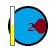
\includegraphics[width=0.13\textwidth]{Abbildungen/RobotinoGZu.png}
    
\includegraphics[width=0.13\textwidth]{Abbildungen/RobotinoDefect.png}
    \includegraphics[width=0.13\textwidth]{Abbildungen/Einhorn.png}
    \caption{Roboter in verschiedenen Stati (vlnr: Greifer offen, Greifer geschlossen, Defekt, Einhorn)}		
    \label{fig:Robotino}
\end{figure}

Nachdem das korrekte Bild für den Robotino ausgewählt wurde wird dieses gleich der Ausrichtung des Robotinos gedreht. In Listing \ref{lst:RobotinoDrehung} ist die Umsetzung im Code zu sehen. Zunächst wird eine Rotationsmatrix rm in Zeile 1 erzeugt. Diese Matrix wird anhand des Winkels des Robotinos konfiguriert. Anschließend wird der Bild des Robotinos in Zeile 3 gedreht und in Zeile 4 angewendet. In Zeile 6 ist die Positionierung des gedrehten Bildes abgebildet. Da die Y-Achse des Robotino invertiert zu der Darstellung ist muss diese als Offset zu 400 angegeben werden. 

\begin{lstlisting}[frame=single, breaklines=true, numbers=left, stepnumber=2, firstnumber=1, numberstyle = \tiny, caption=Robotino Drehung ,label=lst:RobotinoDrehung]
QMatrix rm;
rm.rotate(-newPosition[2]);
QPixmap pixmap = Rlabel->pixmap()->copy().transformed(rm);
Rlabel->setPixmap(pixmap);

Robotino->move(newPosition[0]/10, 400-(newPosition[1]/10));
\end{lstlisting}

Zusätzlich zur Position beinhaltet jeder Robotino in der Mitte eine Zahl, die die eindeutige RoboterID repräsentiert. Somit kann sofort erkannt werden, welcher Robotino dargestellt ist. Außerdem ist an der linken Seite einen Akkustand als vertikaler Balken dargestellt. Der Akkustand ist gleich dem der unten im Roboterstatus-View angezeigt wird und wird dort näher beleuchtet. Am Akkustand am Robotino kann direkt erkannt werden, welcher Robotino welchen Akkustand besitzt ohne erst die IDs abgleichen zu müssen.  

\subsection{Parkplätze und Ladestationen}

Im unteren Bereich der Live-View befinden sich die vier Parkplätze für die Robotinos. Je nach Zustand werden diese verschieden dargestellt. Sobald ein Parkplatz für einen Robotino reserviert wird oder durch einen Robotino belegt ist wird dieser in hellgelb abgebildet. 
Ein freier Parkplatz wird, wie in Abbildung \ref{fig:Parkplatz} rechts, blau dargestellt. 

Eine Aktualisierung erfolgt über den Aufruf der Funktion UpdateParkplatz() in der MainWindow. 

\begin{figure}[htb]
    \centering
    
\includegraphics[width=0.4\textwidth]{Abbildungen/Parkplatz.png}
    \caption{Visualisierung Parkplatz}		
    \label{fig:Parkplatz}
\end{figure}

Wie die Parkplätze werden auch die Ladestationen entweder reserviert (Abb. \ref{fig:Ladestation} oben) in blassem hellgelb dargestellt, oder in kräftigem Gelb für freie Ladestationen (Abb. \ref{fig:Ladestation} unten). 

\begin{figure}[htb]
    \centering
    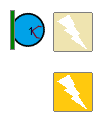
\includegraphics[width=0.25\textwidth]{Abbildungen/Laden.png}
    \caption{Visualisierung Ladestation}		
    \label{fig:Ladestation}
\end{figure}

\subsection{Stationen}

Die Stationen enthalten Informationen über die Werkstücke, die an ihnen bearbeitet werden. Es gibt insgesamt 8 Stationen, wobei immer zwei Stationen horizontal zusammengefasst sind. Ein solcher Stationsverbund ist in Abbildung \ref{fig:Station} abgebildet. Der oberste Kreis einer Station repräsentiert den RFID-Kopf. Darunter befinden sich die beiden Arbeitsplätze. Jeder Arbeitsplatz enthält in seiner Farbkodierung eine Information über das Werkstück. In der Abbildung sind alle möglichen Farbkodierungen dargestellt.

\begin{figure}[htb]
    \centering
    
\includegraphics[width=0.18\textwidth]{Abbildungen/Station.png}
    \caption{Stationen mit verschiedenen Arbeitsplatzstati}		
    \label{fig:Station}
\end{figure}

Sobald ein Arbeitsplatz reserviert wird, da sich ein Werkstück auf dem Weg dahin befindet ist dieser Gelb dargestellt. Ein roter Arbeitsplatz zeigt an, das dieser defekt ist und nicht mehr angefahren werden kann. Ein defekter Arbeitsplatz wird von der Auftragsplanung nicht mehr berücksichtigt. Diese Einstellung kann mit der Hard-Code Area erzeugt werden. Wenn ein Werkstück an den Arbeitsplatz abgelegt wird befindet sich dieses in Bearbeitung und der Platz wird Orange dargestellt. Sobald die Bearbeitung abgeschlossen ist wechselt die Farbe des Arbeitsplatz auf grün und das Werkstück ist bereit zur Abholung. Ein leerer Arbeitsplatz wird in neutralem grau dargestellt. 

Über die Funktion UpdateStationsplatz() kann die Farbkodierung eines einzelnen Arbeitsplatz anhand des übergebenen Status angepasst werden. 

Zusätzlich zu den Arbeitsplatzstati wird neben jeder Station angezeigt, ob diese reserviert ist. Da nicht zwei Robotinos gleichzeitig zu einer Station fahren sollen, werden diese, sobald sich ein Robotino auf dem Weg dahin befindet oder an einer Station arbeitet, reserviert. Eine reservierte Station ist in der Visualisierung an dem hellgelben X neben der Station zu erkennen. In Abbildung \ref{fig:Station} ist die linke Station reserviert und die rechte Station frei. Mit der Funktion UpdateStation() kann die Reservierung für eine Station angepasst werden. 

Im Normalbetrieb, ohne die Zusatzfunktionalität der Hard-Code Area, bewirkt ein Klick auf einen Arbeitsplatz eine Aktualisierung der Timestamp-Area. 

\section{Auftragsübersicht}
\label{sec:Auftragsuebersicht}
on_AuftragsListWidget_itemClicked
on_AuftragsListWidget_itemDoubleClicked
AddAuftragsItem

on_pushButton_clicked
on_pushButton_2_clicked
on_Pause_clicked
on_ButtonAuftragBlocked_clicked

\begin{figure}[htb]
    \centering
    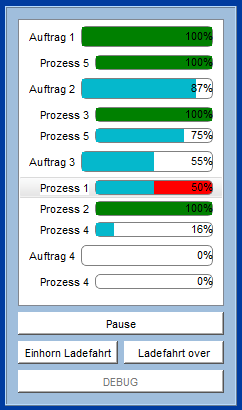
\includegraphics[width=0.4\textwidth]{Abbildungen/Auftragsfortschritt.png}
    \caption{Auftragsfortschritt}		
    \label{fig:Auftragsfortschritt}
\end{figure}

\begin{figure}[htb]
    \centering
    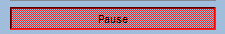
\includegraphics[width=0.4\textwidth]{Abbildungen/Pause.png}
    \caption{Pause Button gedrückt}		
    \label{fig:Pause}
\end{figure}

\section{Tab-View}

\subsection{Log-View}

WriteToDebugTextArea
Alle Logtypen beschreiben!

\begin{figure}[htb]
    \centering
    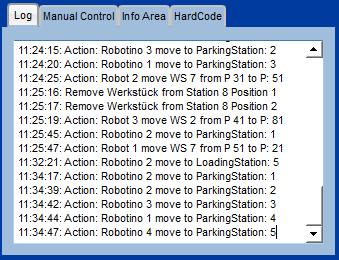
\includegraphics[width=0.6\textwidth]{Abbildungen/Log.png}
    \caption{Tab: Log View}		
    \label{fig:Log}
\end{figure}

\subsection{Manual Control}

on_S8P2weg_clicked...

\begin{figure}[htb]
    \centering
    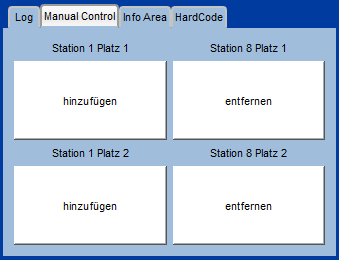
\includegraphics[width=0.6\textwidth]{Abbildungen/ManualControl.png}
    \caption{Tab: Manual Control}		
    \label{fig:ManualControl}
\end{figure}

\subsection{Timestamp-Area}

Wann wird was angezeigt? man muss...

SetTimestamps
StationClicked
\begin{figure}[htb]
    \centering
    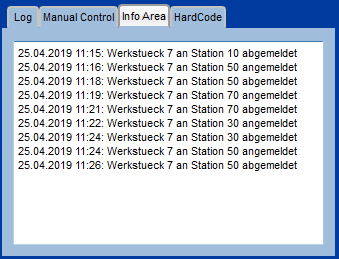
\includegraphics[width=0.4\textwidth]{Abbildungen/TimestampsWerkstueck.png}
    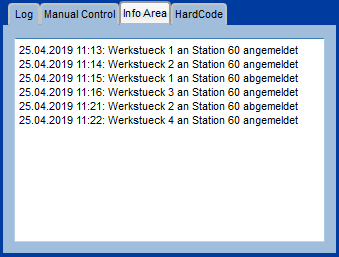
\includegraphics[width=0.4\textwidth]{Abbildungen/TimestampsStation.png}
    \caption{Tab: Info Area}		
    \label{fig:InfoArea}
\end{figure}

\subsection{Hard-Code Bereich}
\label{sec:HardCode}
GetPressedHardCodeButton
ResetButtonsExeptOne
on_ButtonDefektPlatz_clicked...
RobotClicked
ParkplatzClicked
\begin{figure}[htb]
    \centering
    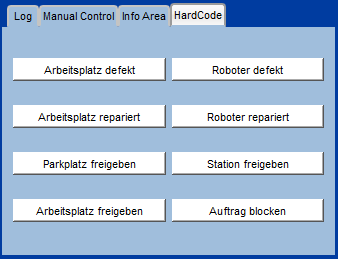
\includegraphics[width=0.6\textwidth]{Abbildungen/HardCode.png}
    \caption{Tab: Hard-Code}		
    \label{fig:HardCode}
\end{figure}

\begin{figure}[htb]
    \centering
    \includegraphics[width=1\textwidth]{Abbildungen/GesamtprogrammROT.png}
    \caption{Übersicht Visualisierung im Hard-Code Modus}		
    \label{fig:GesamtprogrammROT}
\end{figure}

\section{Roboterstatus}

In Bereich IV wird der Status jedes Robotinos dargestellt. Dabei ist auf der linken Seite der Alive-Status der Robotinos, und auf der rechten Seite der Akkustand dargestellt (Abb. \ref{fig:Batterie}). 

\begin{figure}[htb]
    \centering
    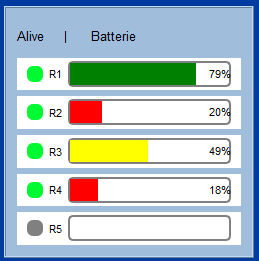
\includegraphics[width=0.5\textwidth]{Abbildungen/Batterie.png}
    \caption{Batterie und Statusanzeige}		
    \label{fig:Batterie}
\end{figure}

\subsection{Akkustand}

Innerhalb der MainWindow wird die Funktion UpdateRobotinoAkku genutzt, um den Akkustand zu aktualisieren. Dabei wird unterschieden, wie hoch der Akkustand ist. Bei einem Akkustand von kleiner als 30 Prozent wird der Fortschrittsbalken rot eingefärbt (Abb. \ref{fig:Batterie} R2, R4). Der Robotino wird bei <25 Prozent Akku zur Ladestation geschickt. 

Ein Akkustand von über 77 Prozent wird, wie in Abbildung \ref{fig:Batterie} R1, grün dargestellt. Bei einem Akkustand zwischen 30 und 77 Prozent wird der Fortschrittsbalken gelb dargestellt (Abb. \ref{fig:Batterie} R3). 

Die Anpassung der Farbe geschieht über das Setzen des Stylesheet für den Fortschrittsbalken. In Listing \ref{lst:ProgressbarStylesheet} ist das implementierte Stylesheet für alle Fortschrittsbalken dargestellt. 

\begin{lstlisting}[frame=single, breaklines=true, numbers=left, stepnumber=2, firstnumber=1, numberstyle = \tiny, caption=Progressbar Stylesheet ,label=lst:ProgressbarStylesheet]
QProgressBar {
    border: 2px solid grey;
    border-radius: 5px;
	text-align: right;
 }

 QProgressBar::chunk {
     background-color: #05B8CC;
     width: 2px;
 }

font: 8pt "OpenSans";
background-color: rgb(160 ,190, 220);
\end{lstlisting}

Indem der in Listing \ref{lst:AkkuStylesheet} dargestellte Code in der UpdateRobotinoAkku() Funktion ausgeführt wird, wird die Farbe des jeweiligen Fortschrittsbalken-Chunk überschrieben und somit angepasst. In Zeile 1 erfolgt die Aktualisierung des Fortschrittsbalken in der Roboterstatus-View. Zeile 2 zeigt die anschließende Aktualisierung des vertikalen Fortschrittsbalken am Robotino. 

\begin{lstlisting}[frame=single, breaklines=true, numbers=left, stepnumber=2, firstnumber=1, numberstyle = \tiny, caption=Stylesheet Aktualisierung der Akku-Progressbar ,label=lst:AkkuStylesheet]
P->setStyleSheet("QProgressBar::chunk {background-color: green}");
Pklein->setStyleSheet("QProgressBar::chunk {background-color: green}");
\end{lstlisting}

\subsection{Alive-Status}

Der linke Bereich des Roboterstatus-View enthält die Information zum Alive-Status des Robotinos (vgl. \ref{sec:Robotino}). Die dargestellte grüne LED blinkt während der Roboter als "`lebend"' gilt. Das blinken ist in Abbildung \ref{fig:Led} abgebildet. 

\begin{figure}[htb]
    \centering
    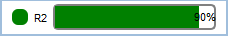
\includegraphics[width=0.4\textwidth]{Abbildungen/BatterieAlive1.png}
    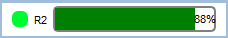
\includegraphics[width=0.4\textwidth]{Abbildungen/BatterieAlive2.png}
    \caption{Roboterstatus-LED blinkend}		
    \label{fig:Led}
\end{figure}

Über die Funktion UpdateRobotinoAlive() kann die LED aktiviert oder deaktiviert werden. Wenn der Roboter nicht mehr "`lebend"' ist wird eine Meldung an das Log geschrieben und die LED grau gesetzt (Abb. \ref{fig:Batterie} R5). 


Über den internen blink-Timer wird alle 500 ms die Funktion ToggleAliveRobotino() aufgerufen. In dieser Funktion wird für alle Robotinos, die "`lebend"' sind, die LED zwischen hellgrün und dunkelgrün gewechselt. Dies geschieht über eine Anpassung des Stylesheets von der LED (siehe Listing \ref{lst:LEDtoggle}). 

\begin{lstlisting}[frame=single, breaklines=true, numbers=left, stepnumber=2, firstnumber=1, numberstyle = \tiny, caption=Stylesheet Aktualisierung der Alive-LED ,label=lst:LEDtoggle]
toggler ? AliveR1->setStyleSheet("QPushButton {background-color: rgb(0,250,50); border-radius: 6px;}") : AliveR1->setStyleSheet("QPushButton {background-color: green; border-radius: 6px;}");
\end{lstlisting}

\section{Prozesseingabe}
\label{sec:Prozesseingabe}

on_sendProzess_clicked

\begin{figure}[htb]
    \centering
    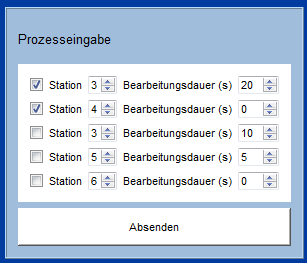
\includegraphics[width=0.5\textwidth]{Abbildungen/Prozesseingabe.png}
    \caption{Visualisierung - Prozesseingabe}		
    \label{fig:Prozesseingabe}
\end{figure}

\section{Auftragseingabe}
\label{sec:Auftragseingabe}

AddAuftragsItem
on_sendAuftrag_clicked

\begin{figure}[htb]
    \centering
    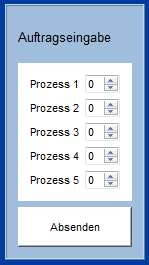
\includegraphics[width=0.25\textwidth]{Abbildungen/Auftragsvergabe.png}
    \caption{Visualisierung - Auftragsvergabe}		
    \label{fig:Auftragsvergabe}
\end{figure}


\section{Benutzerinteraktion}

\subsection{Tooltips}
\label{sec:tooltips}
UpdateStationToolTip
\inlinetodo {Tooltips mit Bildern her und erklaeeeren}

\section{MainWindow}

Neben allen bisher bereits beschriebenen Funktionen wird folgend eine Übersicht über die MainWindow-Funktion gegeben. 

